%% LaTeX2e class for student theses
%% sections/content.tex
%%
%% Karlsruhe University of Applied Sciences
%% Faculty of  Computer Science and Business Information Systems
%% Distributed Systems (vsys)
%%
%% Prof. Dr. Christian Zirpins
%% christian.zirpins@hs-karlsruhe.de
%%
%%
%% Version 0.2, 2017-11-15
%%
%% --------------------------------------------------------
%% | Derived from sdqthesis by Erik Burger burger@kit.edu |
%% --------------------------------------------------------
\chapter{ 
	\iflanguage{english}{Introduction}{Einleitung}
}
\label{ch:Introduction}
\iflanguage{english}{
	\todo{- Justification of this work}
	Centralization of data and trust in individual instances is ubiquitous today. In the Internet there is a wealth of social networks such as Facebook, Twitter, Google+, Instagram or Pinterest which mostly retain the right to the data you get from their users and last but not least sell this data for advertising purposes. It is also easier for criminals and secret services to access the entire database, since centralised networks usually also have a central database or access point. When the access to this central point is reached, the whole database can be read.\\
	
	What does decentralized mean? In politics, decentralization \glqq is the transfer of central government tasks to subnational or subsidiary level(s)\grqq\cite{wikipedia-decentralization-politics}. In the energy industry, one speaks of \glqq decentralized power generation\grqq if the power is also generated at the places where it is consumed. An example of this would be a hydroelectric power plant that supplies electricity to the surrounding villages or cities\cite{wikipedia-decentralization-energy}. In computer science, decentralization means the distribution of data over several independent servers. \\
	
	By allocating tasks to sub-national or subsidiary levels, the central government level is relieved of its burden and thus has more resources for other tasks. When hydroelectric power plants are built close to villages and towns, there is no need to transport electricity over long distances, which reduces the loss of electricity when it is transported over the power grid. Decentralisation of social networks brings various advantages. One advantage is the scalability of decentralized social networks. By adding more instances, new resources can be made available to the network. Another advantage is that there is no central control body that can be corrupted by criminals, economic lobbyists or government authorities.\\
	
	% - Goal of the work
	The aim of the work is to implement the distributed server-to-server protocol as a prototype and to test the security standards for the ActivityPub protocol recommended by the \gls{w3c} community. In addition, the work should give an overview of the basics of the protocol and how the relevant components are to be understood. The security standards used relate to the authentication of the client against the server and additionally the server to each other, as well as ensuring the manipulation-free transmission of content.\\

}{
	Zentralisierung von Daten und das Vertrauen auf einzelne Instanzen ist heutzutage allgegenwärtig. Im Internet gibt es eine Fülle an sozialen Netzwerken wie Facebook, Twitter, Google+, Instagram oder Pinterest die zumeist das Recht an den Daten, die Sie von ihren Nutzer bekommen, behalten und nicht zuletzt diese Daten auch verkaufen für z. B. Werbezwecke. Für Kriminelle sowie Geheimdienste ist es außerdem leichter an die gesamte Datenbank zu kommen, da bei zentralisierten Netzwerken meist auch eine zentrale Datenbank, bzw. ein zentraler Zugriffspunkt, vorhanden ist. Wenn der Zugriff auf diesen zentralen Punkt erreicht ist kann die ganze Datenbank ausgelesen werden. Um die Kontrolle über Daten in Richtung Nutzer zu lenken kann dezentralisiert werden. Dadurch werden auch mehrere unabhängig administrierte Datenbanken benötigt, was die Sicherheit des Netzwerks erhöht.\\
	
	Was bedeutet nun dezentral? In der Politik wird unter Dezentralisierung \glqq die Übertragung zentral staatlicher Aufgaben auf subnationale oder subsidiäre Ebene(n) verstanden\grqq~(Vgl. \cite{bpb-dezentralisierung}). In der Energiewirtschaft spricht man von einer \glqq dezentralen Stromerzeugung\grqq, wenn der Strom an den Stellen wo er verbraucht auch erzeugt wird. Ein Beispiel hierfür wäre ein Wasserkraftwerk, dass den Strom für die umgebenen Dörfer oder Städte liefert (Vgl. \cite{wikipedia-dezentralisierung-energie}). In der Informatik versteht man unter Dezentralisierung das verteilen von u. a. Daten über mehrere unabhängige Server hinweg.\\
	
	Durch die Verteilung der Aufgaben wird die zentral staatliche Ebene entlastet und hat somit mehr Ressourcen für andere Aufgaben. Beim Errichten von Wasserkraftwerken nahe an Dörfern und Städten entfällt der Transport des Stroms über größere Distanzen und somit verringert sich der Verlust beim Transport über das Stromnetz. Dezentralisieren von sozialen Netzwerken bringt verschiedene Vorteile mit sich. Ein Vorteil ist die Skalierbarkeit bei dezentralen sozialen Netzwerken. Durch das hinzufügen weiterer Instanzen können dem Netzwerk neue Ressourcen bereitgestellt werden. Ein weiterer Vorteil liegt darin, dass keine zentrale Kontrollinstanz vorhanden ist welche korrumpiert werden kann, sei es durch Kriminelle, wirtschaftliche Interessenvertreter oder staatliche Autoritäten.\\
	
	Die Arbeit wird in einer gemeinnützigen und durch Spenden finanzierten GmbH namens Human-Connection angefertigt. Hauptsächlicher Arbeitsschwerpunkt der gGmbH\footnote{Gemeinnützige Gesellschaft mit beschränkter Haftung} liegt in der Umsetzung und Verbreitung eines neuartigen sozialen Wissens- und Aktionsnetzwerkes welches seinen Nutzern die Möglichkeit bieten soll von der Information hin zur Aktion zu kommen. Dabei liegt das Augenmerk auf der Gemeinnützigkeit, Transparenz durch Open-Source, deutschen Serverstandorten, Kommerz-, Werbe- und Zensurfreiheit, lösungsorientiertem Handeln sowie verzicht auf Datenverkauf. Ziel der Arbeit ist die Erstellung eines Frameworks zur Integration des förderierten Server-zu-Server Protokolls in eine bestehende Applikation mit möglichst wenig Programmieraufwand. Darüber hinaus soll die Arbeit einen Überblick über die Grundlagen des Protokolls, sowie zugehörigen Standards, geben und wie die relevanten Bestandteile zu verstehen sind.\\
	
	Um sicherzustellen das gesendete Inhalte vom einem zum Anderen Server manipulationsfrei übertragen wurden, wird ein Verfahren benötigt um dies zu gewährleisten. Nicht nur für die manipulationsfreie Übertragung sondern auch das Authentisieren der Nutzer am Empfänger-Server, also das Sicherstellen ob die Inhalte wirklich von einem Nutzer auf einem Server stammen, welcher über den zum öffentlichen Schlüssel zugehörigen privaten Schlüssel zum Verifizieren verfügt, wird ein Verfahren benötigt. Das für die beiden genannten Punkte bei der Implementierung verwendete Verfahren ist das HTTP-Signaturverfahren. Eine Signatur kann mit einem privaten Schlüssel in Kombination mit einer Hashfunktion erstellt werden. Dabei können verschiedene Funktionen zum Signieren sowie Verifizierne verwendet werden.
	
	\section{Motivation}
	\label{sec:Introduction:Motivation}
	Bei zentralen sozialen Netzwerken besitzt die Kontrolle über Daten das Unternehmen. Durch die Dezentralisierung bleiben Daten bei den einzelnen Instanzen des sozialen Netzwerkes. Die Datenbanken bei zentralen Netzwerken können zwar verteilt sein und auch das Netzwerk könnte dezentral angelegt sein, doch die Hoheit über Daten liegt bei dem Unternehmen. Bei zentralen sozialen Netzwerken ist es außerdem nicht ohne weiteres möglich Inhalte mit anderen Netzwerken auszutauschen. Mit einem Protokoll wie ActivityPub wird das Verteilen sowie der Zugriff auf Inhalte und der Austausch von Aktivitäten über mehrere soziale Netzwerke hinweg ermöglicht.\\
	
	Der im März 2018 vom \gls{w3c} empfohlene Standard namens \glqq ActivityPub\grqq~wurde auf Basis des Wissens im Umgang mit dem OStatus und Pump.io Protokoll entwickelt und besteht aus zwei Teilen. Dem Client-zu-Server Protokoll, auch \glqq Social API\grqq~genannt, und dem förderierten Server-zu-Server Protokoll. Durch die ActivityPub \gls{w3c} Empfehlung Anfang 2018 und die \gls{swwg} Arbeitsgruppe des \gls{w3c} sowie weiteren, wird die Verbreitung des Protokolls vorangebracht. Dabei kann der Netzwerkeffekt genutzt werden.\\
	
	Der Netzwerkeffekt ist ein aus der Volkswirtschaftslehre stammender Begriff. Für die Verständlichkeit sei als Beispiel das Telefonnetz genannt:\\
	Umso mehr Leute ein Telefon besitzen, umso höher ist der Nutzen für jeden einzelnen Telefon Besitzer (Vgl. \cite{netzwerkeffekt}).\\
	Übertragen auf ActivityPub bedeutet das soviel wie:\\
	\glqq Je mehr Netzwerke den Standard implementieren, desto höher ist der Nutzen (die Reichweite) für ein einzelnes Netzwerk und im Endeffekt für die einzelnen Nutzer\grqq.\\
	%Der Grundgedanke des World Wide Web nach Tim Beners Lee war es ein offenes und freies Web zu schaffen um Wissen für die Allgemeinheit zugänglich zu machen. \todo{Quelle: Web-Report stelle suchen}
	
	Durch ein Framework zur Integration des ActivityPub Standard kann dieser Effekt verstärkt werden. In dieser Abschlussarbeit wird ein solches Framework erstellt um es Entwicklern leichter zu ermöglichen ihre Applikation ActivityPub konform zu machen.\\
	\begin{figure}[h]
		\begin{minipage}{\textwidth}
			\centering
			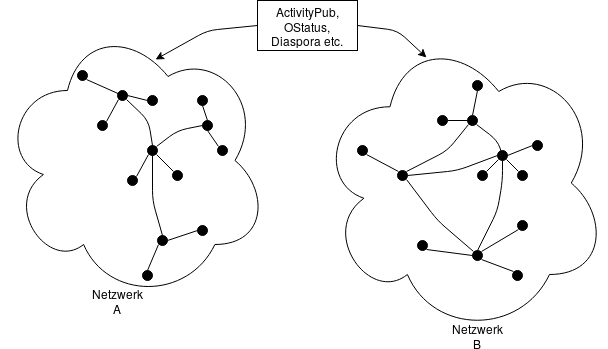
\includegraphics[scale=0.5]{figures/federate.png}
			\label{fig:federate1}
			\caption{Förderieren von Netzwerken über verschiedene Protokolle}
		\end{minipage}
	\end{figure}
	
	Um die Förderierung zweier dezentrale sozialer Netzwerke zu veranschaulichen, wird Abb. 1.1 auf der nächsten Seite betrachtet. In dieser sind zwei Netzwerke zu sehen (Netzwerk A und B). Die Superpeers (Instanzen) eines Netzwerks können, auch wenn dieses noch nicht förderiert wurde, untereinander kommunizieren. Die Regulären Peers stellen hier die einzelnen Clients dar, welche mit dem zugehörigen Superpeer kommunizieren um Inhalte anzuzeigen sowie zu erstellen. Das förderieren der beiden Netzwerke kann über Protokolle wie OStatus (s. \ref{sub:ostatus}) oder ActivityPub erreicht werden. Dabei erhalten Superpeers die Fähigkeit auch mit Superpeers anderer Netzwerke zu interagieren anstatt nur mit denjenigen innerhalb des eigenen Netzwerks.\\
	
	Es wird ein Problemansatz und eine Problemlösung gewählt, welche Entwicklern die Integration des ActivityPub Protokolls so einfach als möglich machen soll. Weder eine extra Datenbank für das Framework, noch viel Vorkenntnis des Protokolls an sich sind notwendig um die Implementierung umzusetzen. Lediglich das Interface muss implementiert werden um einen lauffähigen ActivityPub Service zu erhalten. Dabei werden Hilfsfunktionen bereitgestellt um die Umsetzung möglichst einfach zu gestalten. Zudem wurde auf ein gutes Codeverständnis Wert gelegt.\\
	
	ActivityPub ist wie \glqq OStatus\grqq~ein Protokoll für dezentrale soziale Netzwerke und wird in dieser Abschlussarbeit implementiert und die wichtigsten Komponenten beschrieben.
	
	\section{Problemansatz}
	Folgende Fragestellung wird in dieser Abschlussarbeit behandelt:
	\begin{addmargin}[1cm]{1cm}
		\vspace{0.5cm}
		\textit{Wie wird der Standard möglichst Entwicklerfreundlich implementiert?}
		\vspace{0.5cm}
	\end{addmargin}
	Ein wichtiger Aspekt dabei ist die spontane Generierung aller ActivityPub spezifischen Komponenten, wie dem Aktorenobjekt, Sammlungen sowie Objekten und Aktivitäten. Dadurch wird keine zusätzliche Datenbank ausschließlich für das Framework benötigt. Es reicht somit die Nutzung einer bestehenden Datenquelle der Applikation.\\
	
	Ein weiterer wichtiger Aspekt liegt in der Schaffung eines Interfaces. Über die Implementierung dieses Interfaces sollen Entwickler in der Lage sein ActivityPub in ihre Applikation zu integrieren. Zur weiteren Vereinfachung wird außerdem eine Sammlung von Hilfsfunktionen erstellt.\\
	
	Außerdem wird auf das Codeverständnis Wert gelegt, was heißt dass die Benennung von Funktionen und Variablen auf eine Weise geschieht die für andere Entwickler auch ohne Dokumentation möglichst leicht verständlich ist.\\
	
	Als letzter Aspekt wird darauf geachtet, dass die Applikation in einen bestehenden Server integriert sowie als eigenständiger Server gestartet werden kann.
	
	\section{Problemlösung}
	Um die spontane Generierung zu erreichen, werden die einzelnen Komponenten als Generator Funktionen implementiert welche die Parameter der Funktion in ein Objekt Literal, mit unter anderem statischen Werten, eintragen.\\
	
	Aufgeteilt wird das Framework in drei Schichten, der Controller-, Service- sowie Datenschicht. Die zu implementierende Schicht ist die Datenschicht. Da in JavaScript Interfaces nativ nicht existieren, wird stattdessen ein Objekt mit leeren Funktionsrümpfen dafür genutzt. Dadurch wird der Fokus des Entwicklers auf die Anbindung der Datenquelle gelenkt. Im besten Falle muss somit nichts in den anderen Schichten, oder auch Hilfsfunktionen, angepasst werden. Allerdings sind Änderungen nötig wenn weitere Aktivitäten und Objekte verarbeitet werden sollen.
}

\section{Struktur der Arbeit}
	%% Kapitel 2
	Kapitel zwei gibt einen Überblick über allgemeine Grundlagen von sozialen Netzwerken. Es wird grob erläutert für was soziale Netzwerke gedacht sind, der Unterschied zwischen zentralen, verteilten, dezentralen und förderierten sozialen Netzwerken herausgestellt sowie auf Sicherheitsaspekte eingegangen. Es wird das Wort Fediverse etwas näher definiert und erläutert worum es sich dabei handelt und im weiteren werden mehrere Protokolle die, sowie auch ActivityPub, zum Fediverse gehören vorgestellt.\\
	
	Im Anschluss wird ein Kryptographie Unterkapitel eingeführt in dem die benötigten Verfahren für die sichere Umsetzung erläutert werden. Begonnen wird mit einer kurzen Einführung in Kryptographie. Darauf folgend wird kurz das RSA Verfahren sowie eine allgemeine Beschreibung von Signatur Algorithmen vorgenommen. HTTP Signaturen werden ausführlicher beschrieben, da diese bei der Implementierung des Prototypen verwendet wurden.\\ 
	
	Darauf folgend wird der ActivityPub Standard eingeführt sowie eingeordnet, Bestandteile des Protokolls beschrieben, die Funktionsweise der Client-zu-Server sowie Server-zu-Server Kommunikation und zugehörige Standards kurz erläutert. Des weiteren wird auf die Authentifizierung und Datenintegrität bei ActivityPub eingegangen um damit folgende Fragen zu klären:
	\begin{itemize}
		\item Wie authentifiziert sich ein Benutzer gegenüber dem Server?
		\item Wie stellt man sicher, dass die übertragenen Daten unverändert angekommen sind?
	\end{itemize}
	%% Kapitel 3
	Zu Beginn von Kapitel drei wird auf die Anforderungen, welche an das Framework gestellt werden eingegangen. Im zweiten Unterkapitel wird dann die Entwurfsentscheidung besprochen und dabei folgende Frage beantwortet:
	\begin{itemize}
		\item Warum wurde die Architektur gewählt?
	\end{itemize}
	Das dritte Unterkapitel gibt Aufschluss über die konkrete technische Architektur. Diese wird anschließend anhand von Diagrammen veranschaulicht und erläutert.\\
	
	%% Kapitel 4
	In Kapitel vier wird die konkrete Implementierung des Prototypen, welcher für das Unternehmen angefertigt wurde in der die Abschlussarbeit bearbeitet wird, erläutert. Anfangs wird die Abfragesprache \glqq GraphQL\grqq~sowie die genutzte Graph-Datenbank des Projekts vorgestellt, für welches die Implementierung angefertigt wird. Danach gibt ein Klassendiagramm der Service- und Datenschicht Aufschluss über die in diesen Objekten enthaltene Funktionalität welche darauf folgend genauer beschrieben wird. Anschließend werden anhand der Verzeichnisstruktur die Controller-Schicht, sowie die Werkzeug und Sicherheitsfunktionalitäten beschrieben. Es werden zusätzlich auch die genutzten Testwerkzeuge und zwei Vorgehensweisen der Softwareentwicklung kurz erläutert. Unterkapitel \ref{sec:server-zu-server-prot} gibt Aufschluss über die implementierte Funktionalität des ActivityPub Standards. Zuletzt wird ein genauerer Blick auf die Signierung sowie Verifikation geworfen.\\
	
	%% Kapitel 5
	Zu Beginn des fünften Kapitels werden verschiedenste Anwendungsbeispiele anhand von Diagrammen veranschaulicht und erklärt. Insgesamt werden die folgenden fünf Anwendungsbeispiele beschrieben:
	\begin{itemize}
		\item Folgen eines Nutzers aus einem anderen Netzwerk
		\item \glqq Liken\grqq~eines Objekts in einem anderen Netzwerk
		\item Rückgängig machen einer zuvor gesendeten \glqq Follow\grqq~Aktivität
		\item Die Umkehrung eines \glqq Likes\grqq~(Dislike)
		\item Artikel erstellen in einem anderen Netzwerk
	\end{itemize}
	Des weiteren wird eine Performanz-Messung für die Signatur Erstellung, sowie Verifikation durchgeführt und die Ergebnisse interpretiert. Bei der Messung werden 4 verschiedene Ergebnistabellen erstellt; Jeweils zwei für eine Hardwarevariation. Zum Einen wird ein älteres Notebook Modell zum testen verwenden, zum Anderen ein Spiele-Computer. Außerdem wird aufgrund der interpretierten Ergebnisse und anderen Aspekten Empfehlungen gegeben, welche Hashfunktion für welchen Zweck am Besten passt.